\documentclass[aspectratio=43,17pt]{beamer} % or 14 or 17 or 20

\usepackage{tikz,pgf,lmodern,textpos,hyperref,graphicx,booktabs,appendixnumberbeamer,cleveref,fancybox,multicol}
\usepackage{pgfcalendar,svg,subfiles,chronosys,cancel,xcolor,color,nth,datenumber,xparse,fp,stackengine,makecell}
\usepackage{enumitem}
\usepackage{marvosym} % \MVRIGHTarrow
\usepackage{amsmath}
\usepackage{centernot}
\usetikzlibrary{positioning}
\usepackage[outline]{contour}
\usepackage[citestyle=authoryear-comp,backend=bibtex]{biblatex}
\usepackage[export]{adjustbox}
\usepackage[en-US]{datetime2}
\usepackage[normalem]{ulem}
\bibliography{references}
\usetheme[numbering=none]{metropolis}

\setlist[itemize]{label={--}}
% \setlist[itemize]{leftmargin=*}

% \bibliography{references}

%!TEX Root = ./presentation.tex

\definecolor{Blue}{HTML}{00548f}
\definecolor{Cardinal Red}{HTML}{8c1515}
\definecolor{White}{HTML}{ffffff}
\definecolor{Cool Grey}{HTML}{4d4f53}
\definecolor{Black}{HTML}{2e2d29}
\definecolor{Bright Red}{HTML}{B1040E}
\definecolor{Dark Red}{HTML}{820000}
\definecolor{Chocolate}{HTML}{2F2424}
\definecolor{Stone}{HTML}{544948}
\definecolor{Fog}{HTML}{F4F4F4}
\definecolor{Light Sandstone}{HTML}{F9F6EF}
\definecolor{Sandstone}{HTML}{d2c295}
\definecolor{Warm Grey}{HTML}{3f3c30}
\definecolor{Beige}{HTML}{9d9573}
\definecolor{Light Sage}{HTML}{c7d1c5}
\definecolor{Clay}{HTML}{5f574f}
\definecolor{Cloud}{HTML}{dad7cb}
\definecolor{Driftwood}{HTML}{b6b1a9}
\definecolor{Stone}{HTML}{928b81}
\definecolor{Sandhill}{HTML}{b3995d}
\definecolor{Palo Alto}{HTML}{175e54}
\definecolor{Teal}{HTML}{00505c}
\definecolor{Purple}{HTML}{53284f}
\definecolor{Redwood}{HTML}{8d3c1e}
\definecolor{Brown}{HTML}{5e3032}
\definecolor{Sky}{HTML}{0098db}
\definecolor{Lagunita}{HTML}{007c92}
\definecolor{Mint}{HTML}{009b76}
\definecolor{Gold}{HTML}{b26f16}
\definecolor{Sun}{HTML}{eaab00}
\definecolor{Poppy}{HTML}{e98300}

\definecolor{USF Green}{HTML}{00543C}
\definecolor{USF Gold}{HTML}{FDBB30}
\definecolor{USF Grey}{HTML}{919194}
% \definecolor{USF }{HTML}{e98300}


\setbeamercolor{normal text}{fg=Black,bg=White}
\hypersetup{colorlinks,linkcolor=USF Green,urlcolor=USF Green,citecolor=USF Green}
% \setbeamercolor{frametitle}{bg=Cardinal Red, fg=Blue}


\setbeamercolor{palette primary}{bg=Fog, fg=USF Green}
\setbeamercolor{palette secondary}{bg=USF Green, fg=Fog}
\setbeamercolor{frametitle}{bg=Fog,fg=USF Green}

% \setbeamercolor{section title}{fg=Dark Red, bg=Fog}
\setbeamercolor{alerted text}{fg=USF Green}

\newcommand{\soutthick}[1]{%
    \renewcommand{\ULthickness}{2.4pt}%
       \sout{#1}%
    \renewcommand{\ULthickness}{.4pt}% Resetting to ulem default
}


  \setbeamercolor{normal text}{%
    fg=Cool Grey,
    bg=White
  }

\setbeamercolor{palette primary}{fg=Fog, bg=Dark Red}
\setbeamercolor{palette secondary}{bg=Dark Red, bg=Fog}
\setbeamercovered{transparent}
% \setbeamercolor{background canvas}{bg=Fog}
\setbeamercolor{frametitle}{bg=Dark Red,fg=Fog}
\hypersetup{colorlinks,linkcolor=Blue,urlcolor=Blue,citecolor=Blue}
\setbeamercolor{alerted text}{fg=Bright Red}
\setbeamertemplate{caption}{\insertcaption}


\setsansfont[BoldFont={Source Sans Pro Bold},
              Numbers={OldStyle}]{Source Sans Pro}
\setmainfont[BoldFont={Source Serif Pro Semibold},
              Numbers={OldStyle}]{Source Serif Pro}
\setmonofont{Source Code Pro}


\metroset{titleformat=smallcaps,numbering=none}


\newenvironment{mystepwiseitemize}{\begin{itemize}[<+-| alert@+>]}{\end{itemize}}




\title{Data Ethics Lecture 3}
\subtitle{recap {\bfseries Promises}\\preview {\bfseries more promises}}
\author[Ali Alkhatib]{{Ali Alkhatib}\\
\href{http://twitter.com/_alialkhatib}{@\_alialkhatib} || \href{mailto:hi@al2.in}{hi@al2.in}}
\date{March 24, 2022}

% \date{\today}


\newcommand{\onlyinsubfile}[1]{#1}
\newcommand{\notinsubfile}[1]{}

\begin{document}
\renewcommand{\onlyinsubfile}[1]{}
\renewcommand{\notinsubfile}[1]{#1}


\begin{frame}
\titlepage
\end{frame}

\begin{frame}[t]\frametitle{Roadmap for today}

\begin{itemize}
    \item Admin?
    \item Recap Promises
    \item Preview other promises (tedious/dangerous \& social good/token stakeholders)
\end{itemize}

\end{frame}

\begin{frame}{admin stuff?}
    
    \begin{itemize}
        \visible<1->{\item reading time/reflection}
        \visible<2->{\item let's do that again \MVRightarrow{}}
    \end{itemize}

\end{frame}


\begin{frame}[plain]

\centering
\emph{check the zoom chat for a link}

\end{frame}


\section{Promises}


\begin{frame}{roadmap}
\begin{itemize}
    \item AI can ``understand'' the world better than we can
    \item AI can make ``fairer'' decisions than we can
\end{itemize}

\end{frame}


%%%%%%%%%%%%%%%%%%%%%%%%%%%%%%
%%%%%%%%%%%%%%%%%%%%%%%%%%%%%%
%%%%%%%%%%%%%%%%%%%%%%%%%%%%%%
%%%%%%%%%%%%%%%%%%%%%%%%%%%%%%
%%%%%%%%%%%%%%%%%%%%%%%%%%%%%%

\section{Understanding}

\begin{frame}[standout]

AI will ``understand'' better than we can

\end{frame}

\begin{frame}{AI will understand more}
    \begin{columns}
    \begin{column}{0.4\textwidth}
    \begin{itemize}[label=\MVRightarrow{}]
    \visible<1->{\item labeling}
    \visible<4->{\item moderation}
    \visible<5->{\item navigation}

    \end{itemize}

    \end{column}
    \begin{column}{0.6\textwidth}
    
    \only<+>{\includegraphics[width=\textwidth]{figures/news/understand/NYT_facebook_primates.png}}

    \only<+>{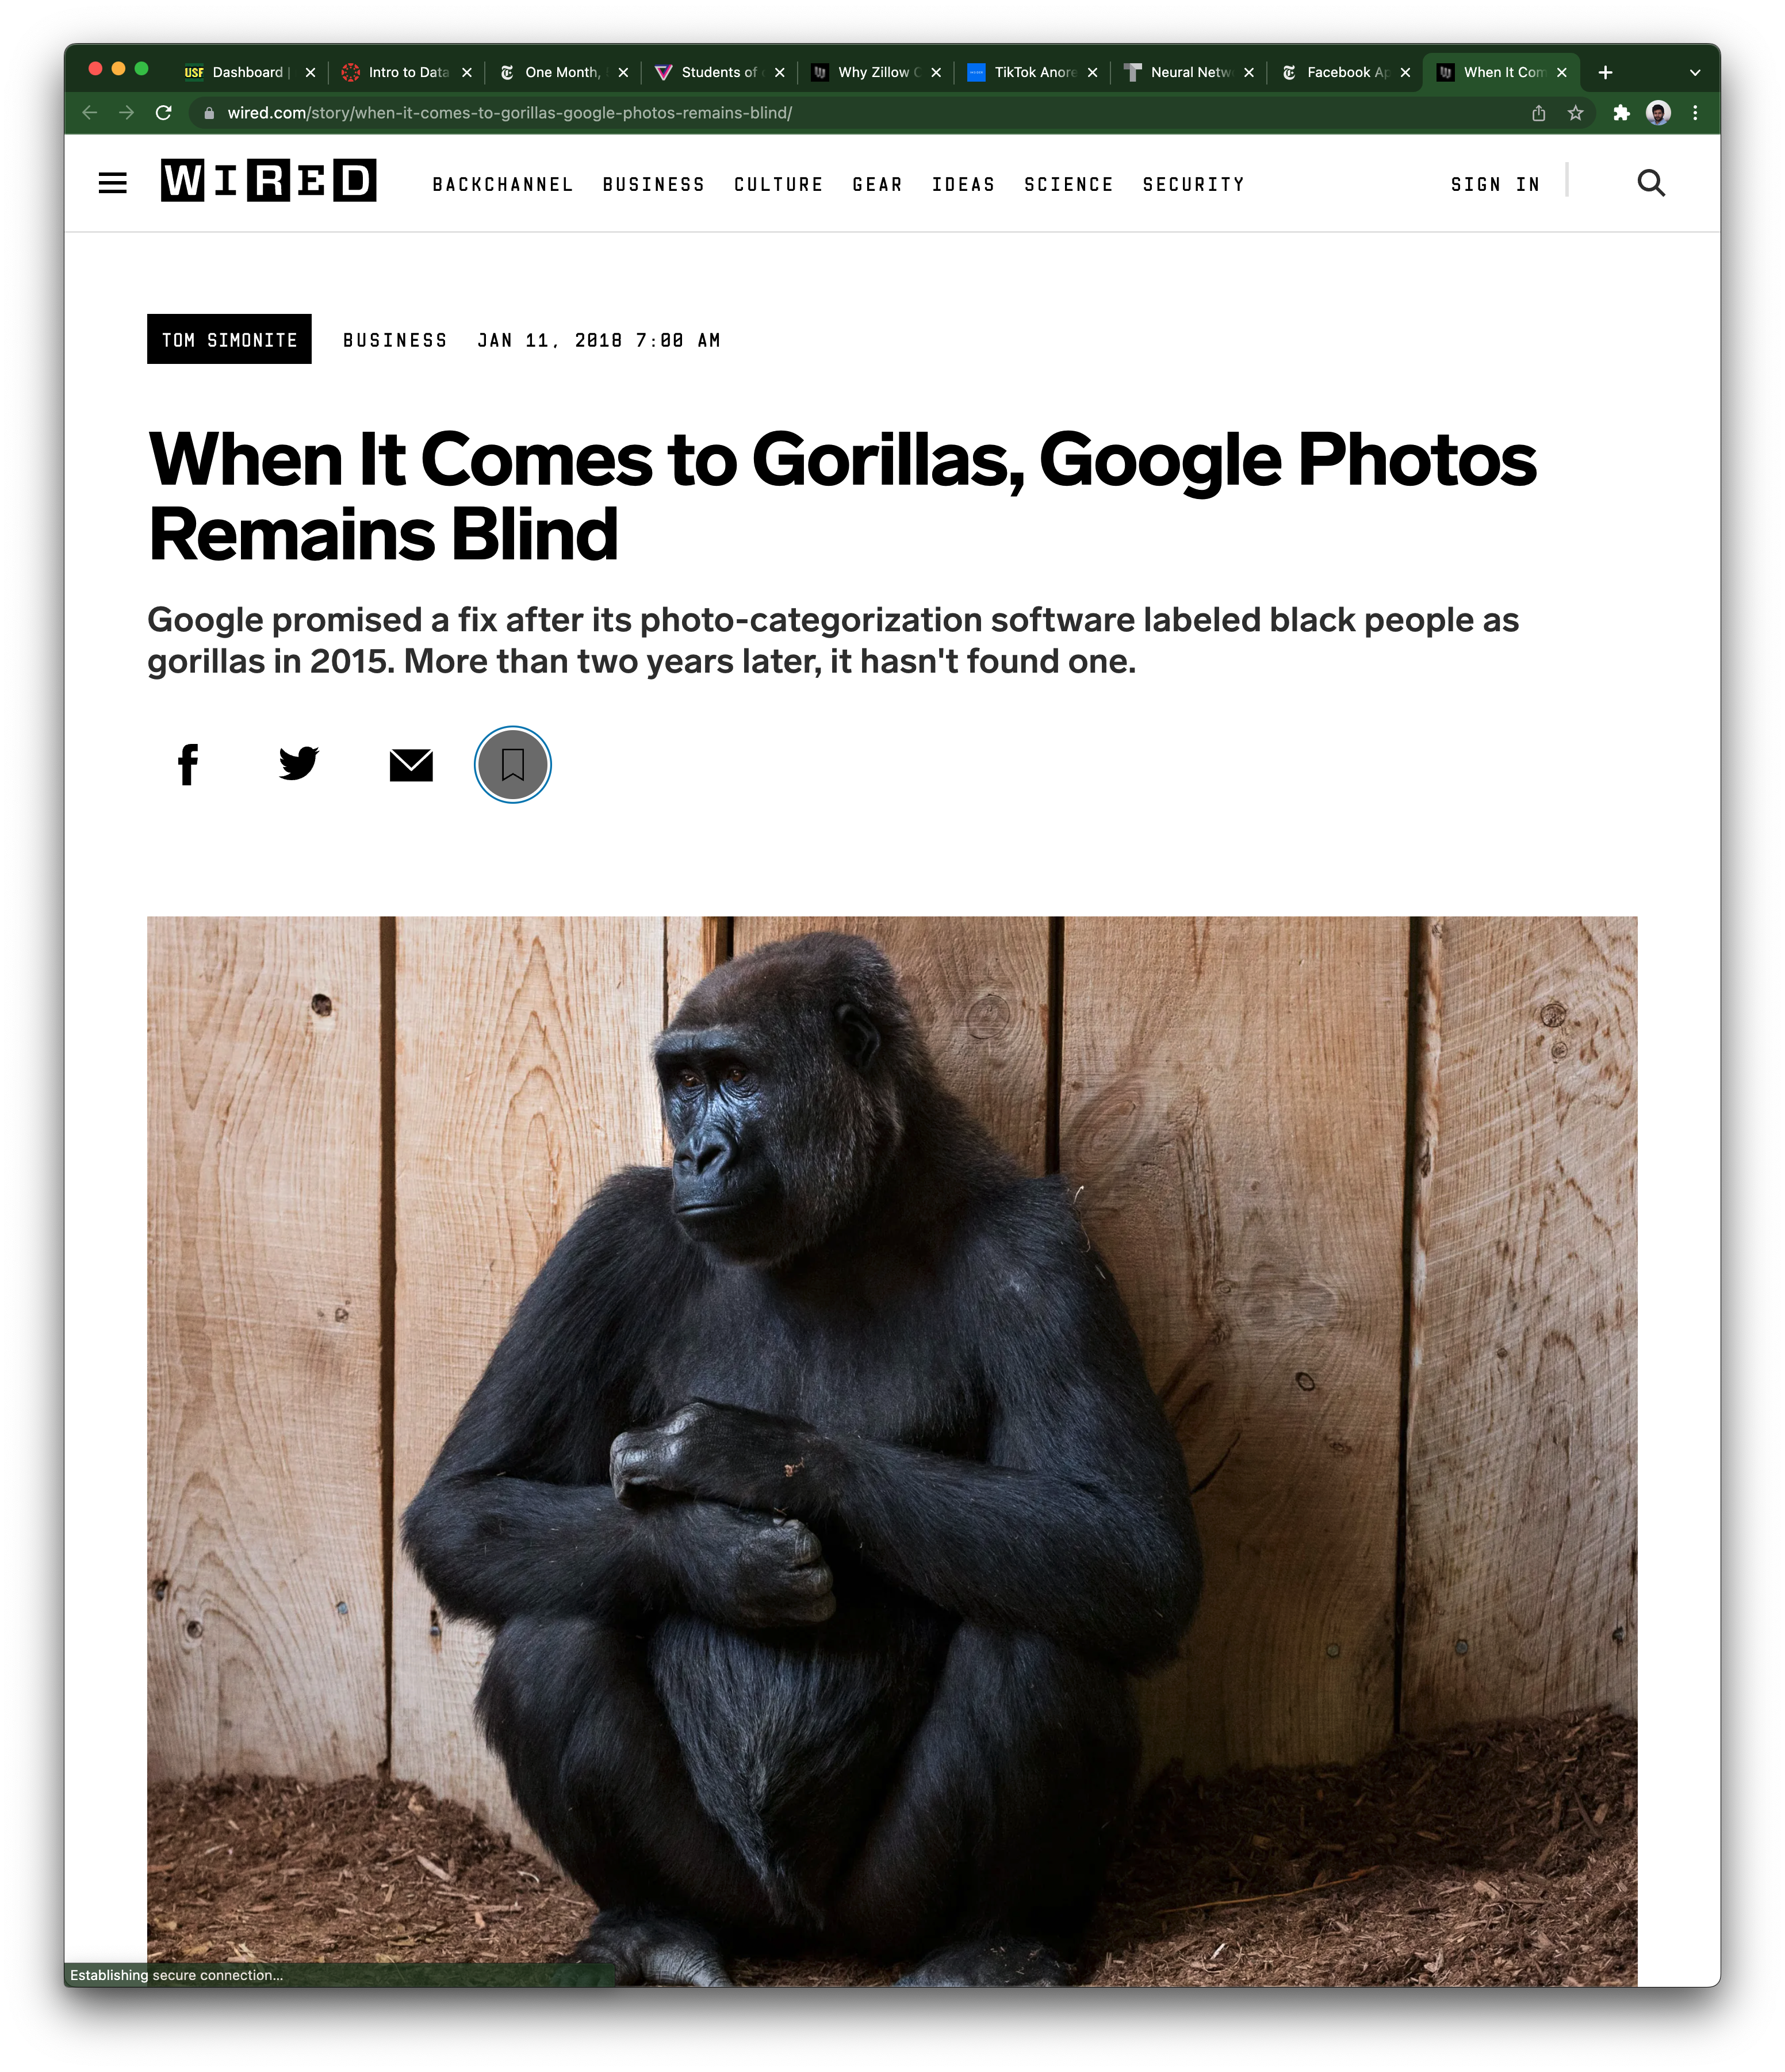
\includegraphics[width=\textwidth]{figures/news/understand/wired_google_gorillas.png}}

    \only<+>{\includegraphics[width=\textwidth]{figures/news/understand/MIT_tech_review_criminals.png}}

    \only<+>{\includegraphics[width=\textwidth]{figures/news/understand/BI_tiktok_anorexia.png}}

    \only<+>{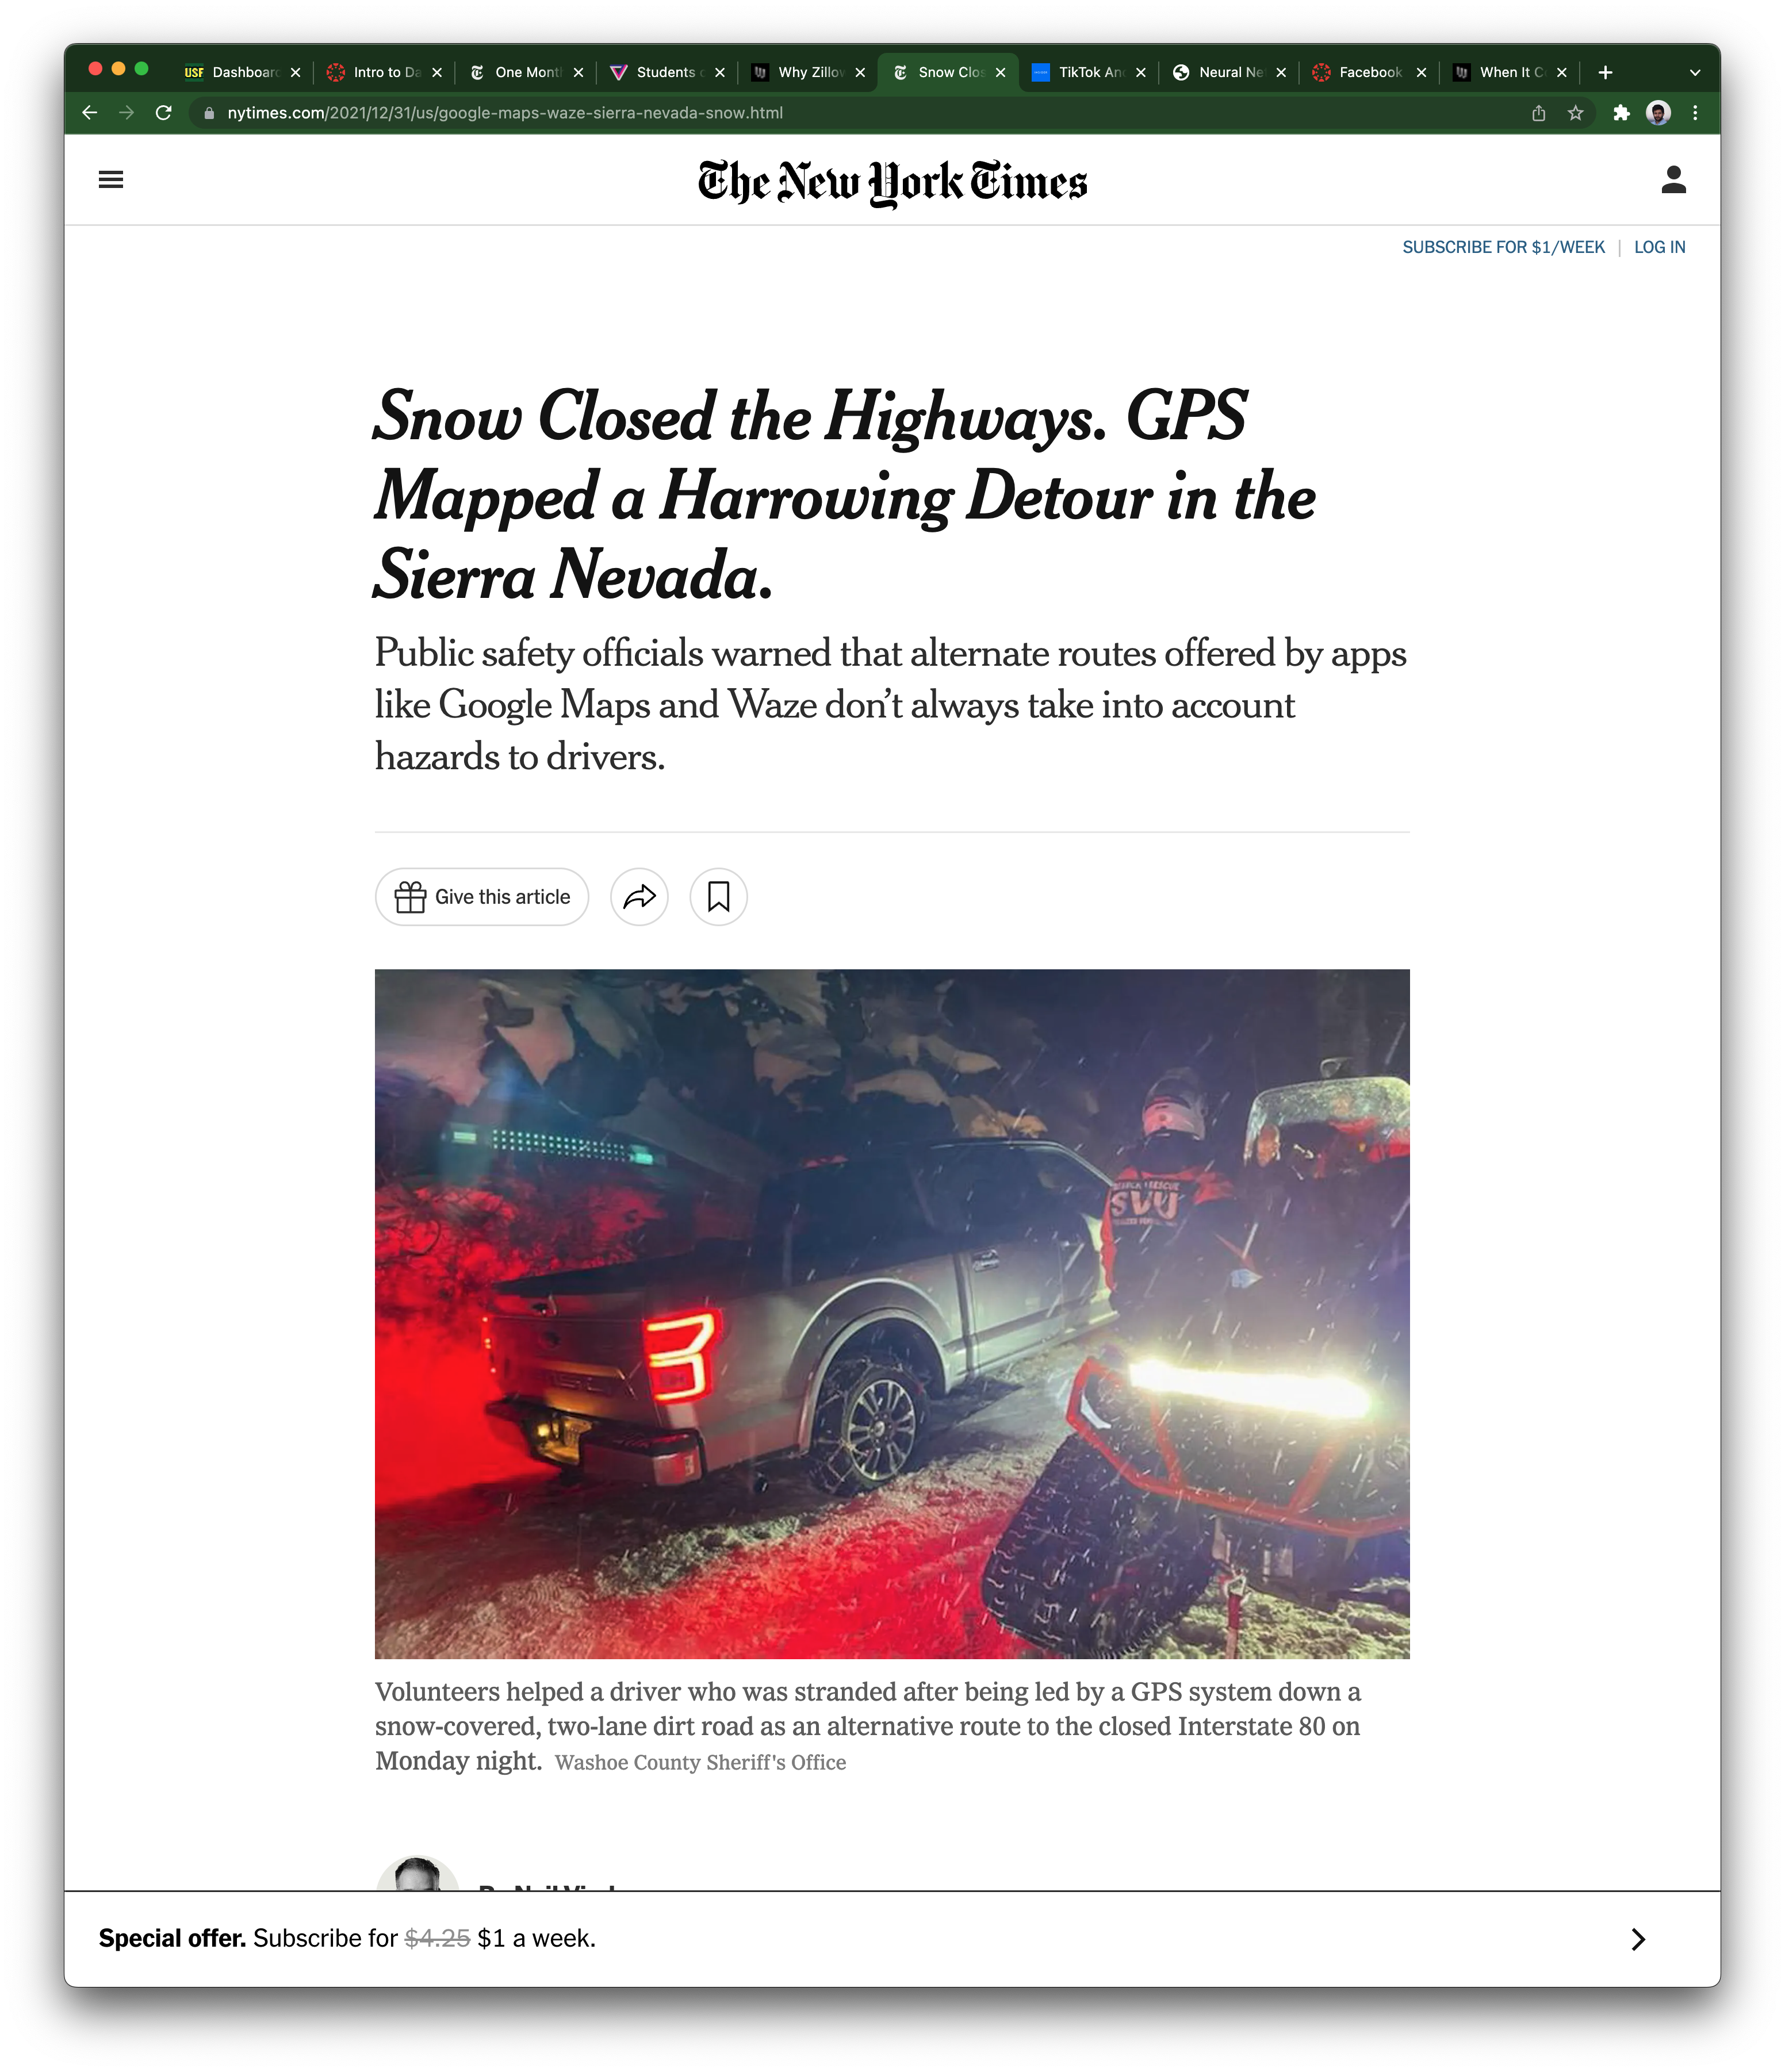
\includegraphics[width=\textwidth]{figures/news/understand/NYT_waze.png}}

    \only<+>{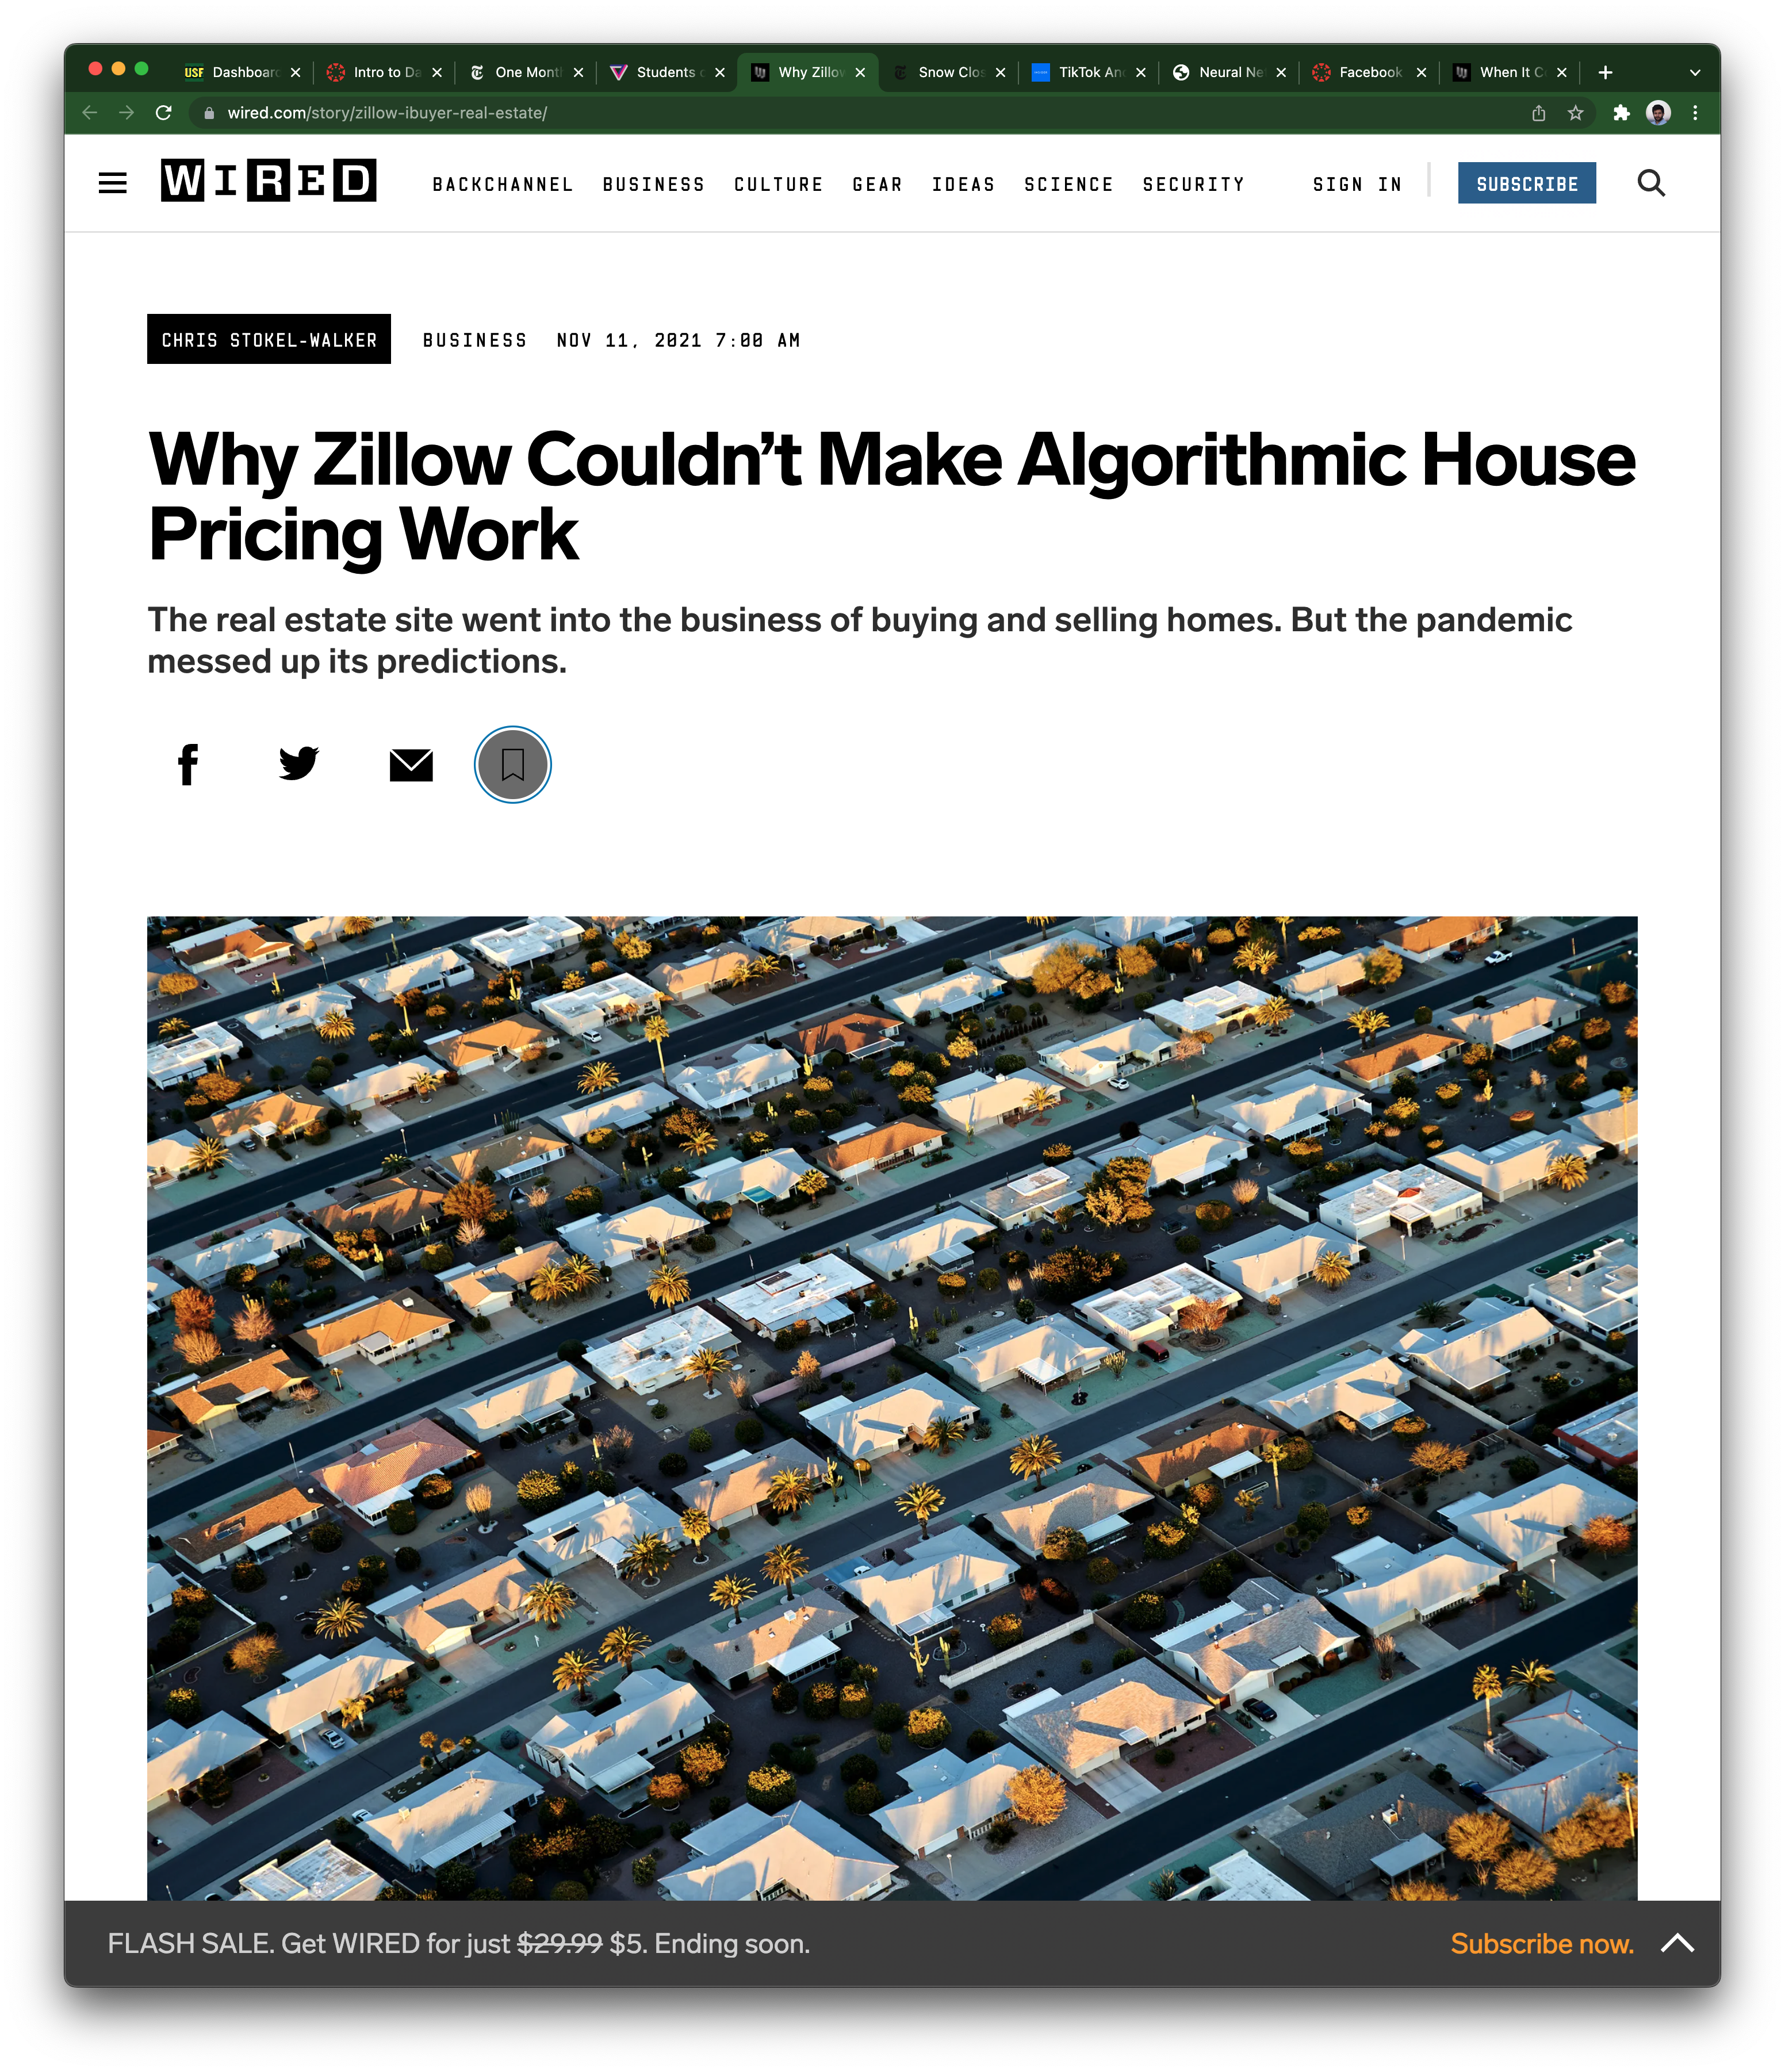
\includegraphics[width=\textwidth]{figures/news/understand/NYT_zillow.png}}

    \only<+>{\includegraphics[width=\textwidth]{figures/news/understand/working_with_machines.png}}

    \only<+>{\includegraphics[width=\textwidth]{figures/news/understand/to_live_in_their_utopia.png}}
    \end{column}
    \end{columns}
\end{frame}

\begin{frame}[standout]
what does it mean to understand something?
\end{frame}

\begin{frame}{understanding}
\centering
\visible<+->{Figuring out what facets you're missing \emph{a priori} is impossible}

\vspace{1em}

\visible<+->{

{\small
How would you \strong{elicit} this dimension as a designer?

What factors prevent or discourage this kind of approach in corporate settings?
}
}

\end{frame}




%%%%%%%%%%%%%%%%%%%%%%%%%%%%%%
%%%%%%%%%%%%%%%%%%%%%%%%%%%%%%
%%%%%%%%%%%%%%%%%%%%%%%%%%%%%%
%%%%%%%%%%%%%%%%%%%%%%%%%%%%%%
%%%%%%%%%%%%%%%%%%%%%%%%%%%%%%

\section{Fairness}

\begin{frame}[standout]

AI will be ``fairer'' or ``more objective'' than we can be

\end{frame}



\begin{frame}{AI will be fairer than we can be}
\begin{columns}
\begin{column}{0.4\textwidth}
\begin{itemize}[label=\MVRightarrow{}]
    \visible<1->{\item medicine}
    \visible<4->{\item education}
    \visible<5->{\item social}

    \end{itemize}
\end{column}
\begin{column}{0.6\textwidth}
\only<+>{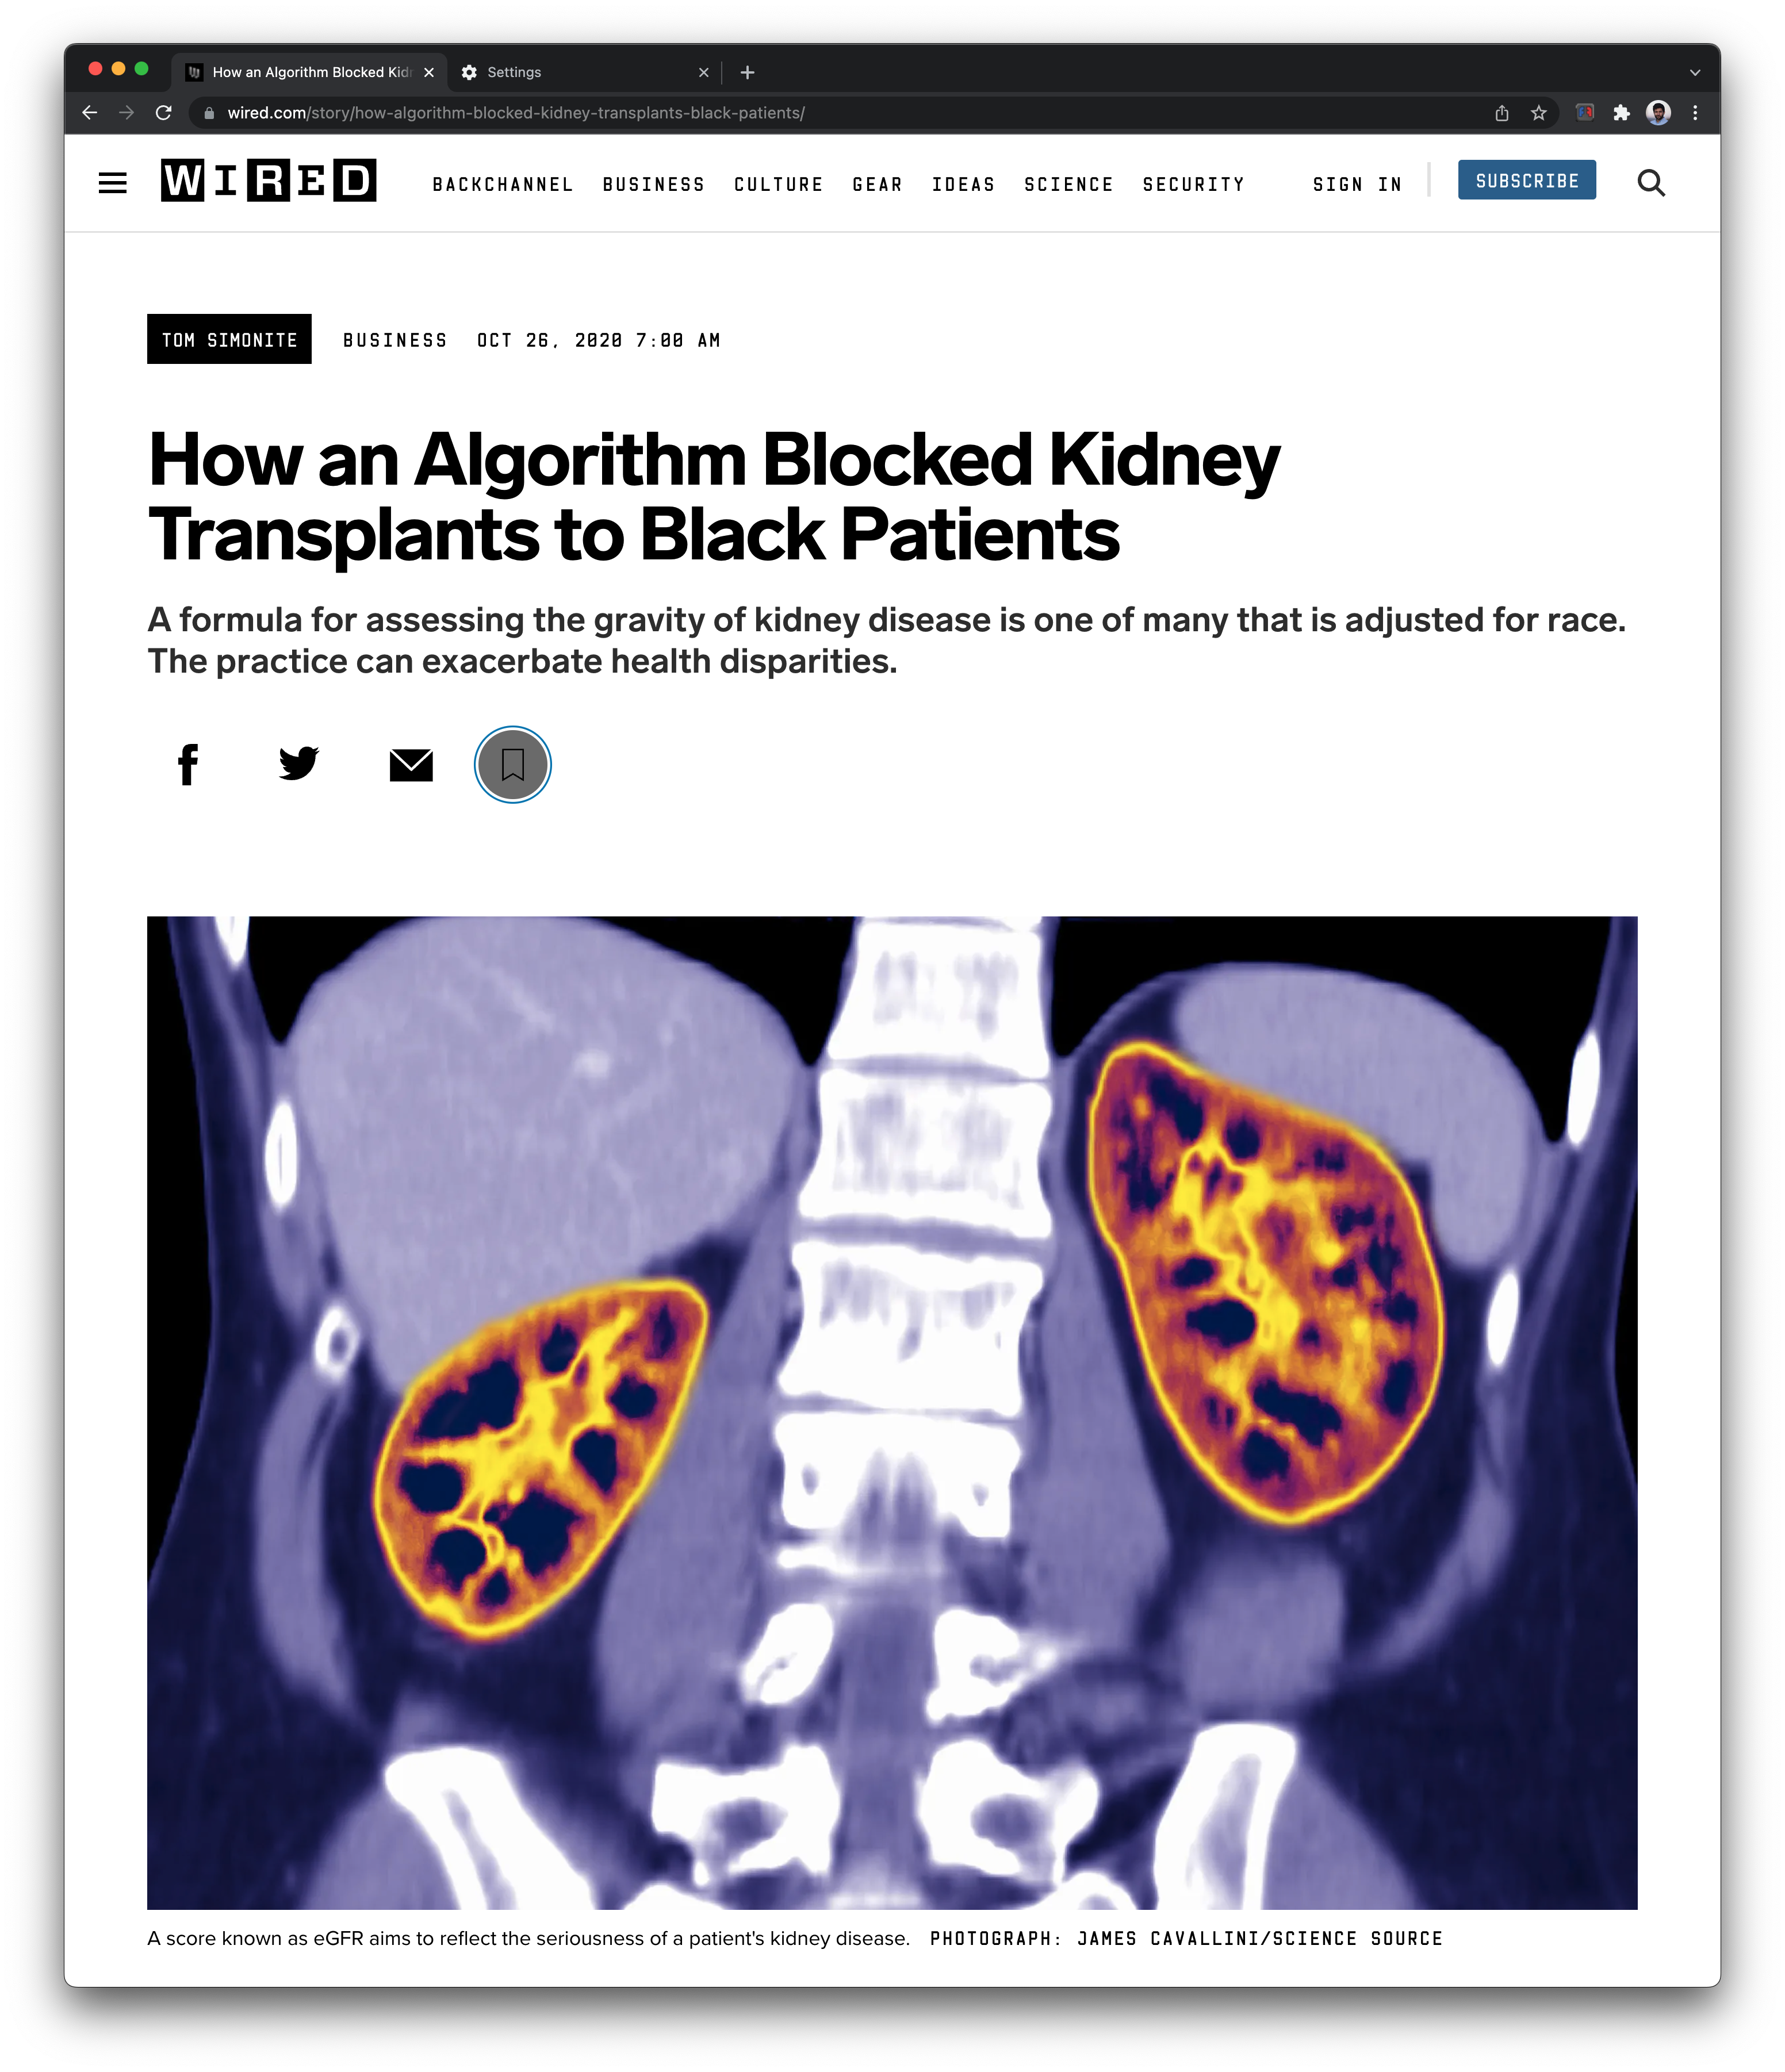
\includegraphics[width=\textwidth]{figures/news/fairer/wired_transplants.png}}

\only<+>{\includegraphics[width=\textwidth]{figures/news/fairer/nature_AI_pain_training.png}}

\only<+>{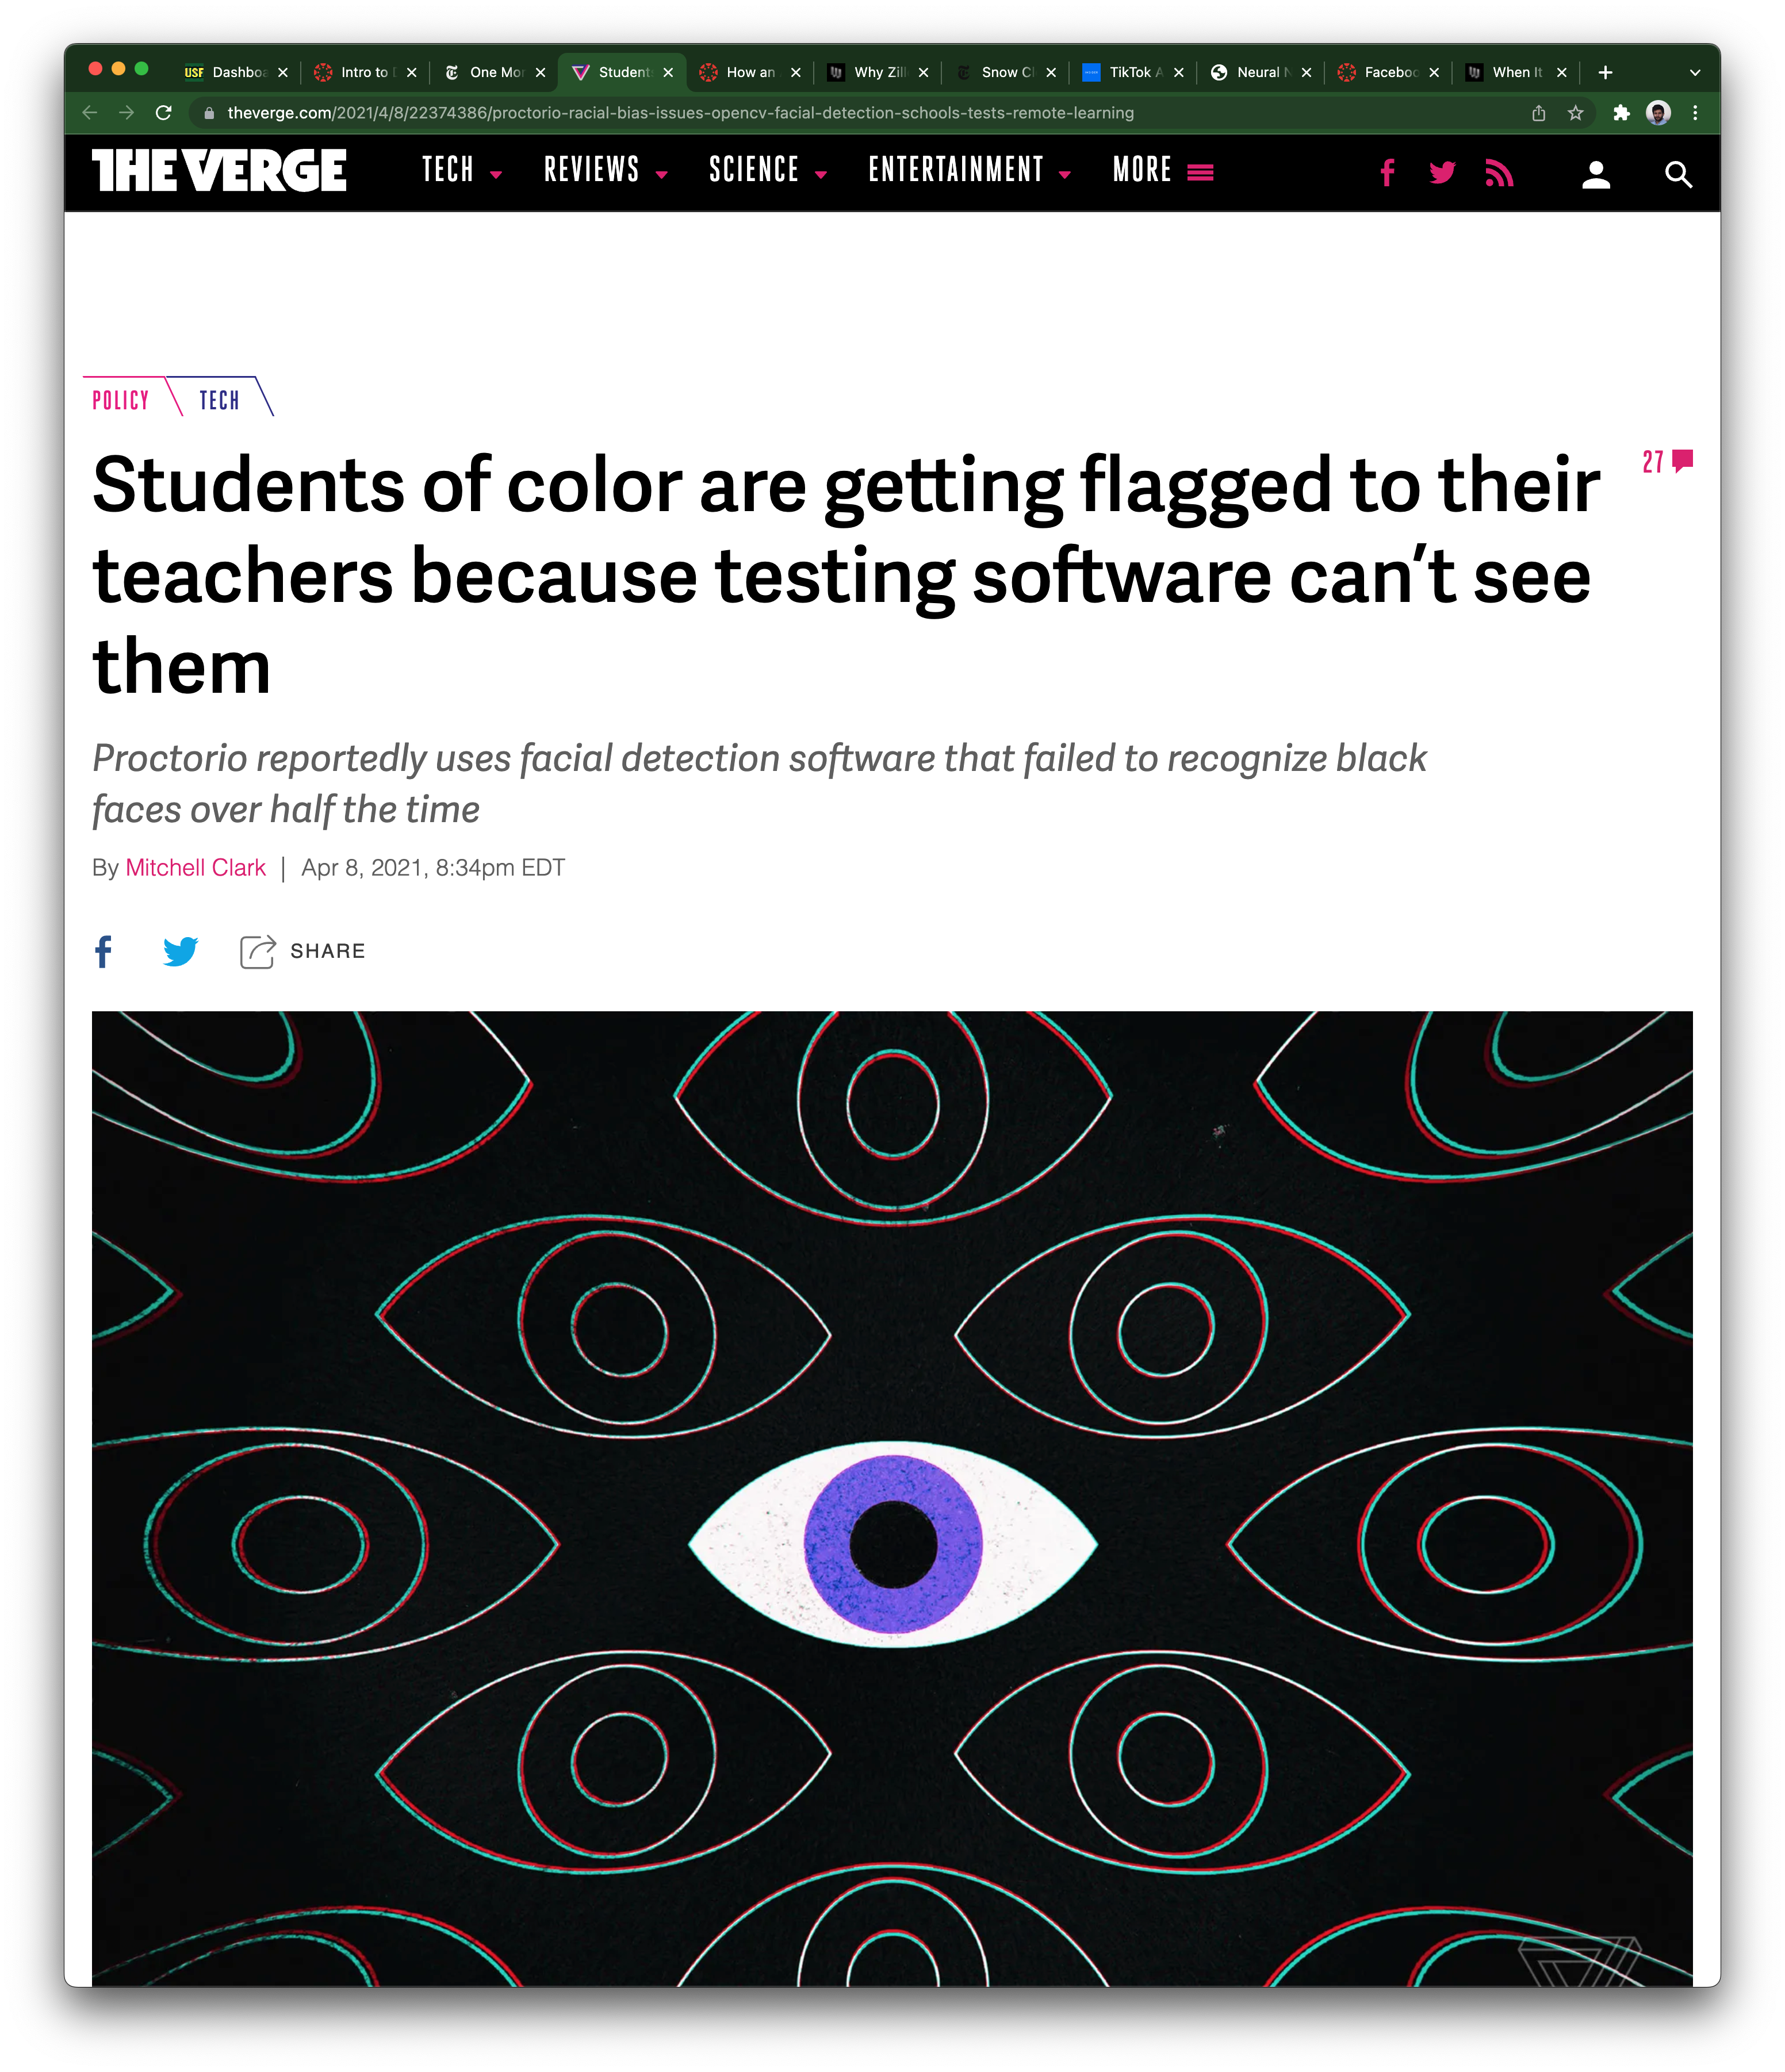
\includegraphics[width=\textwidth]{figures/news/fairer/verge_testing.png}}

\only<+>{
\includegraphics[width=\textwidth]{figures/news/fairer/verge_ditched_exams.png}}

\only<+>{\includegraphics[width=\textwidth]{figures/news/fairer/twitter_image_crop.png}}

\only<+>{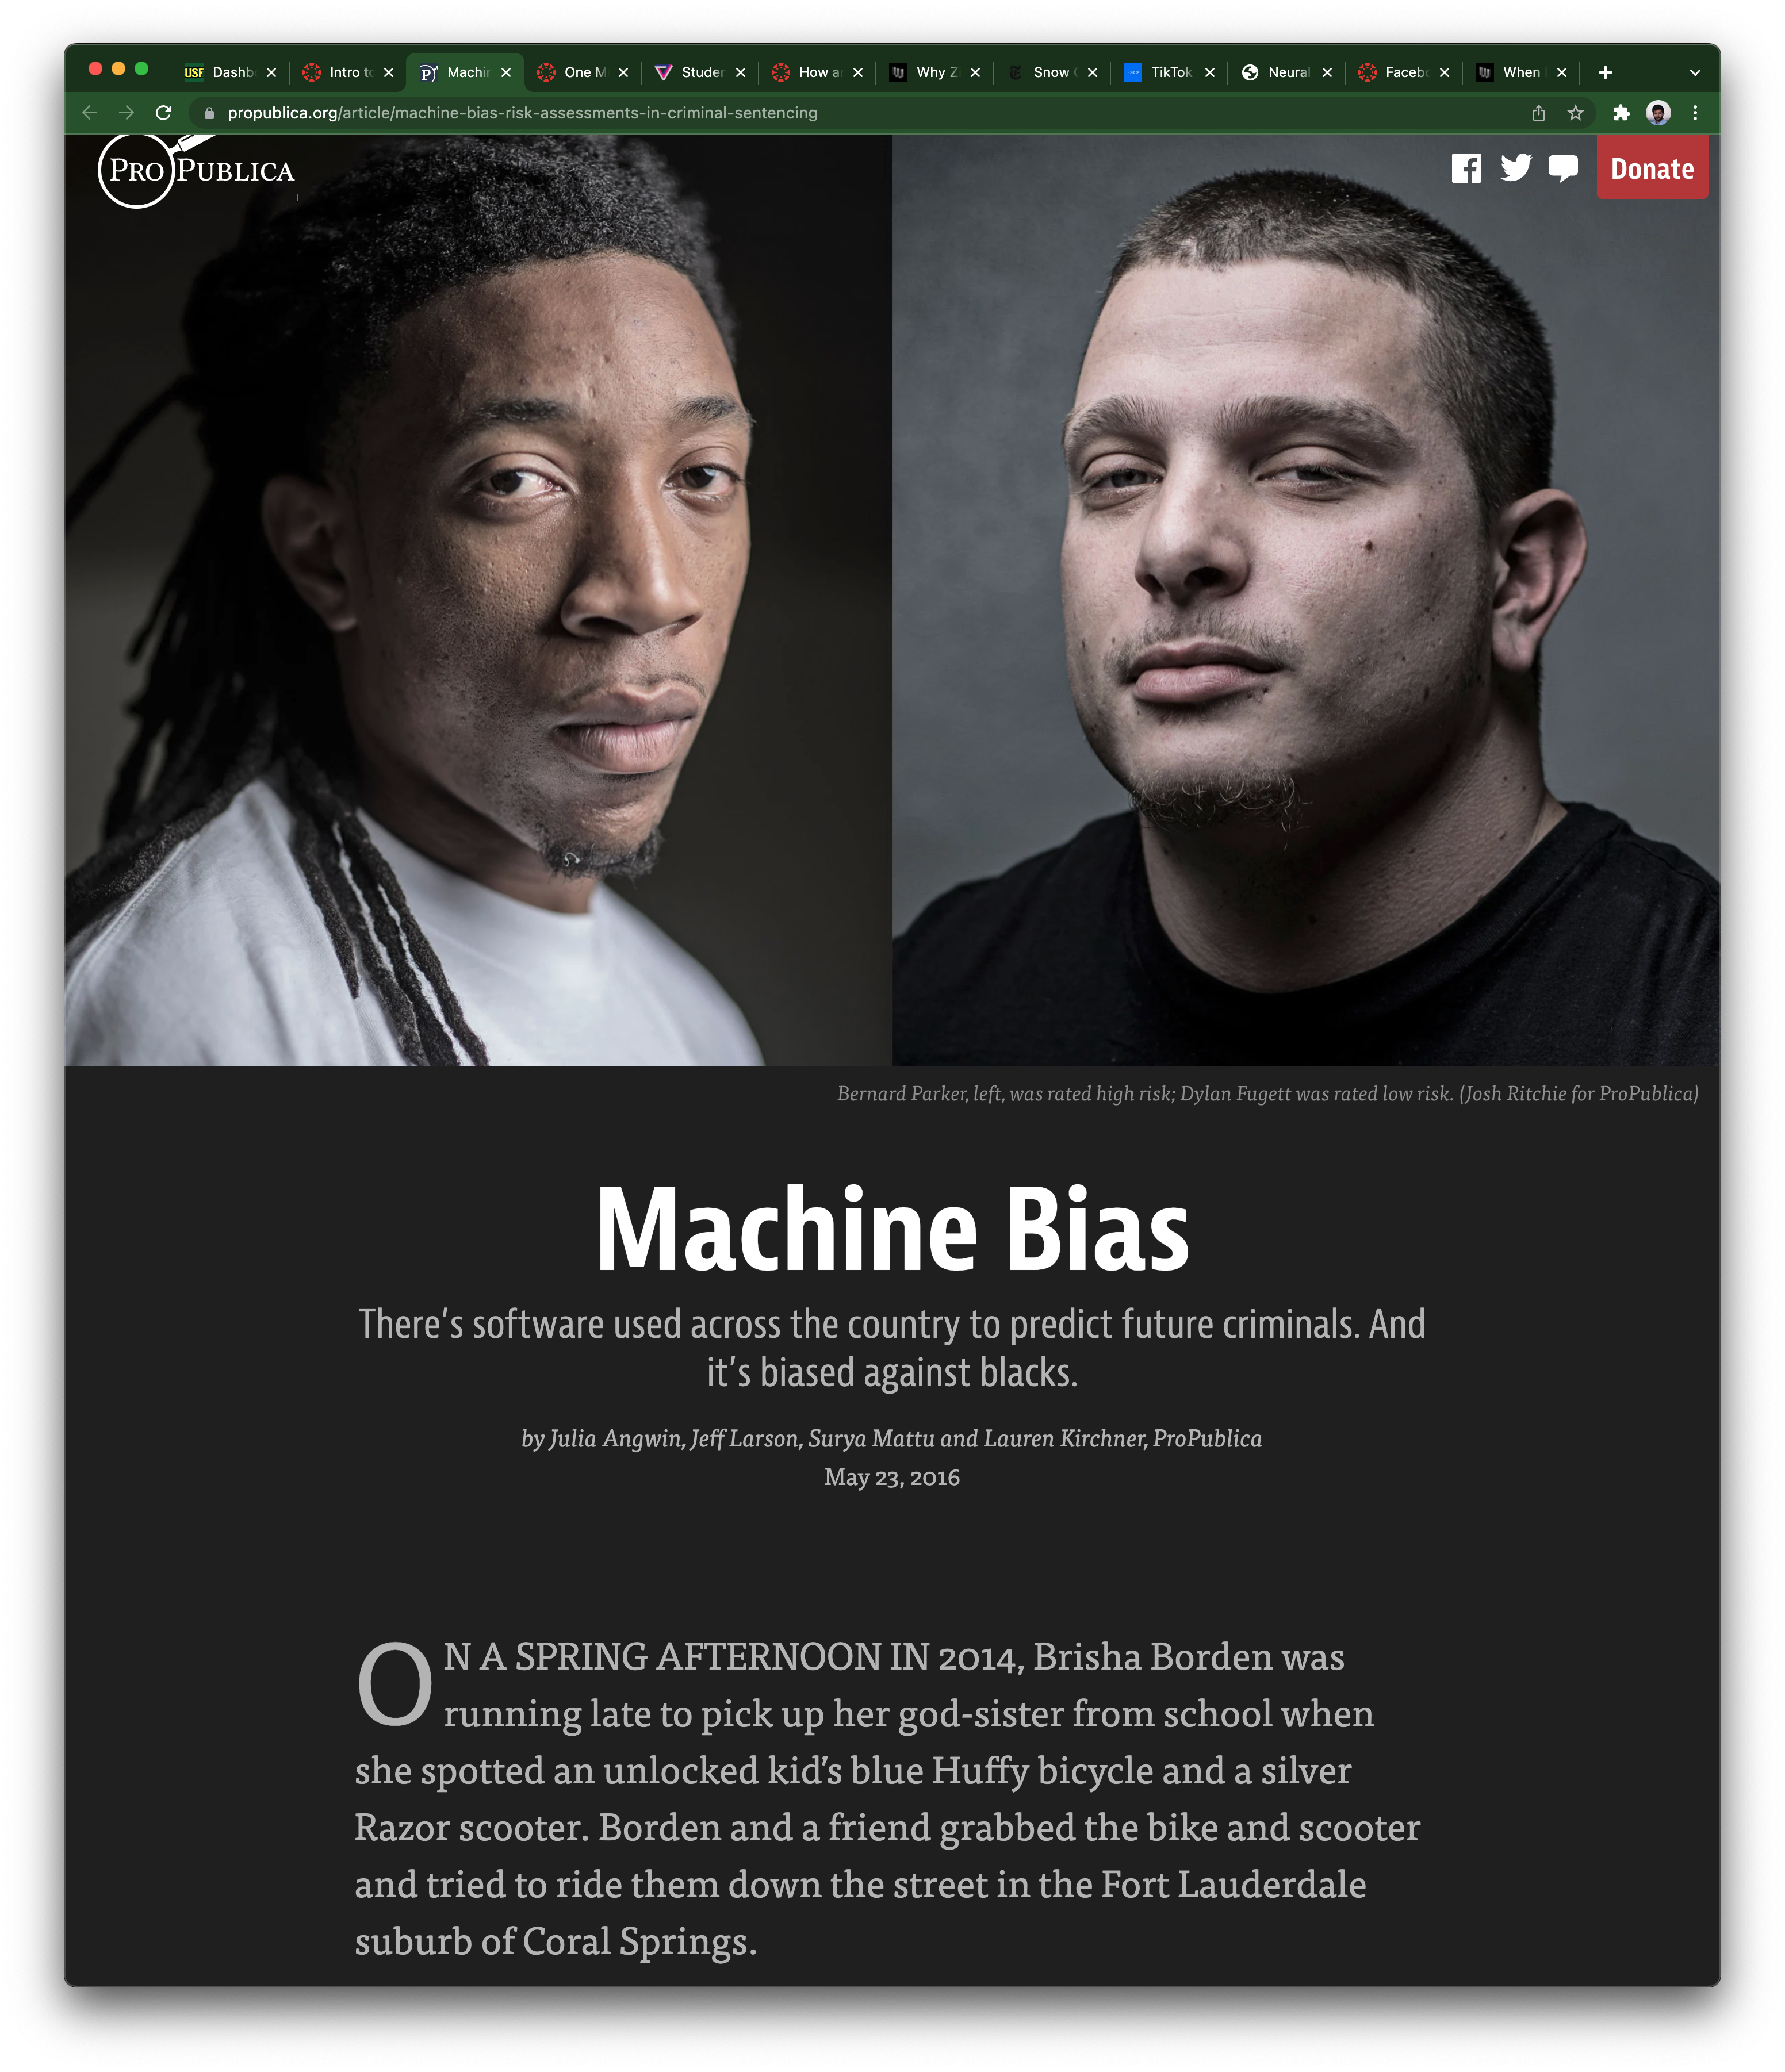
\includegraphics[width=\textwidth]{figures/news/fairer/propublica_bias.png}}

\only<+>{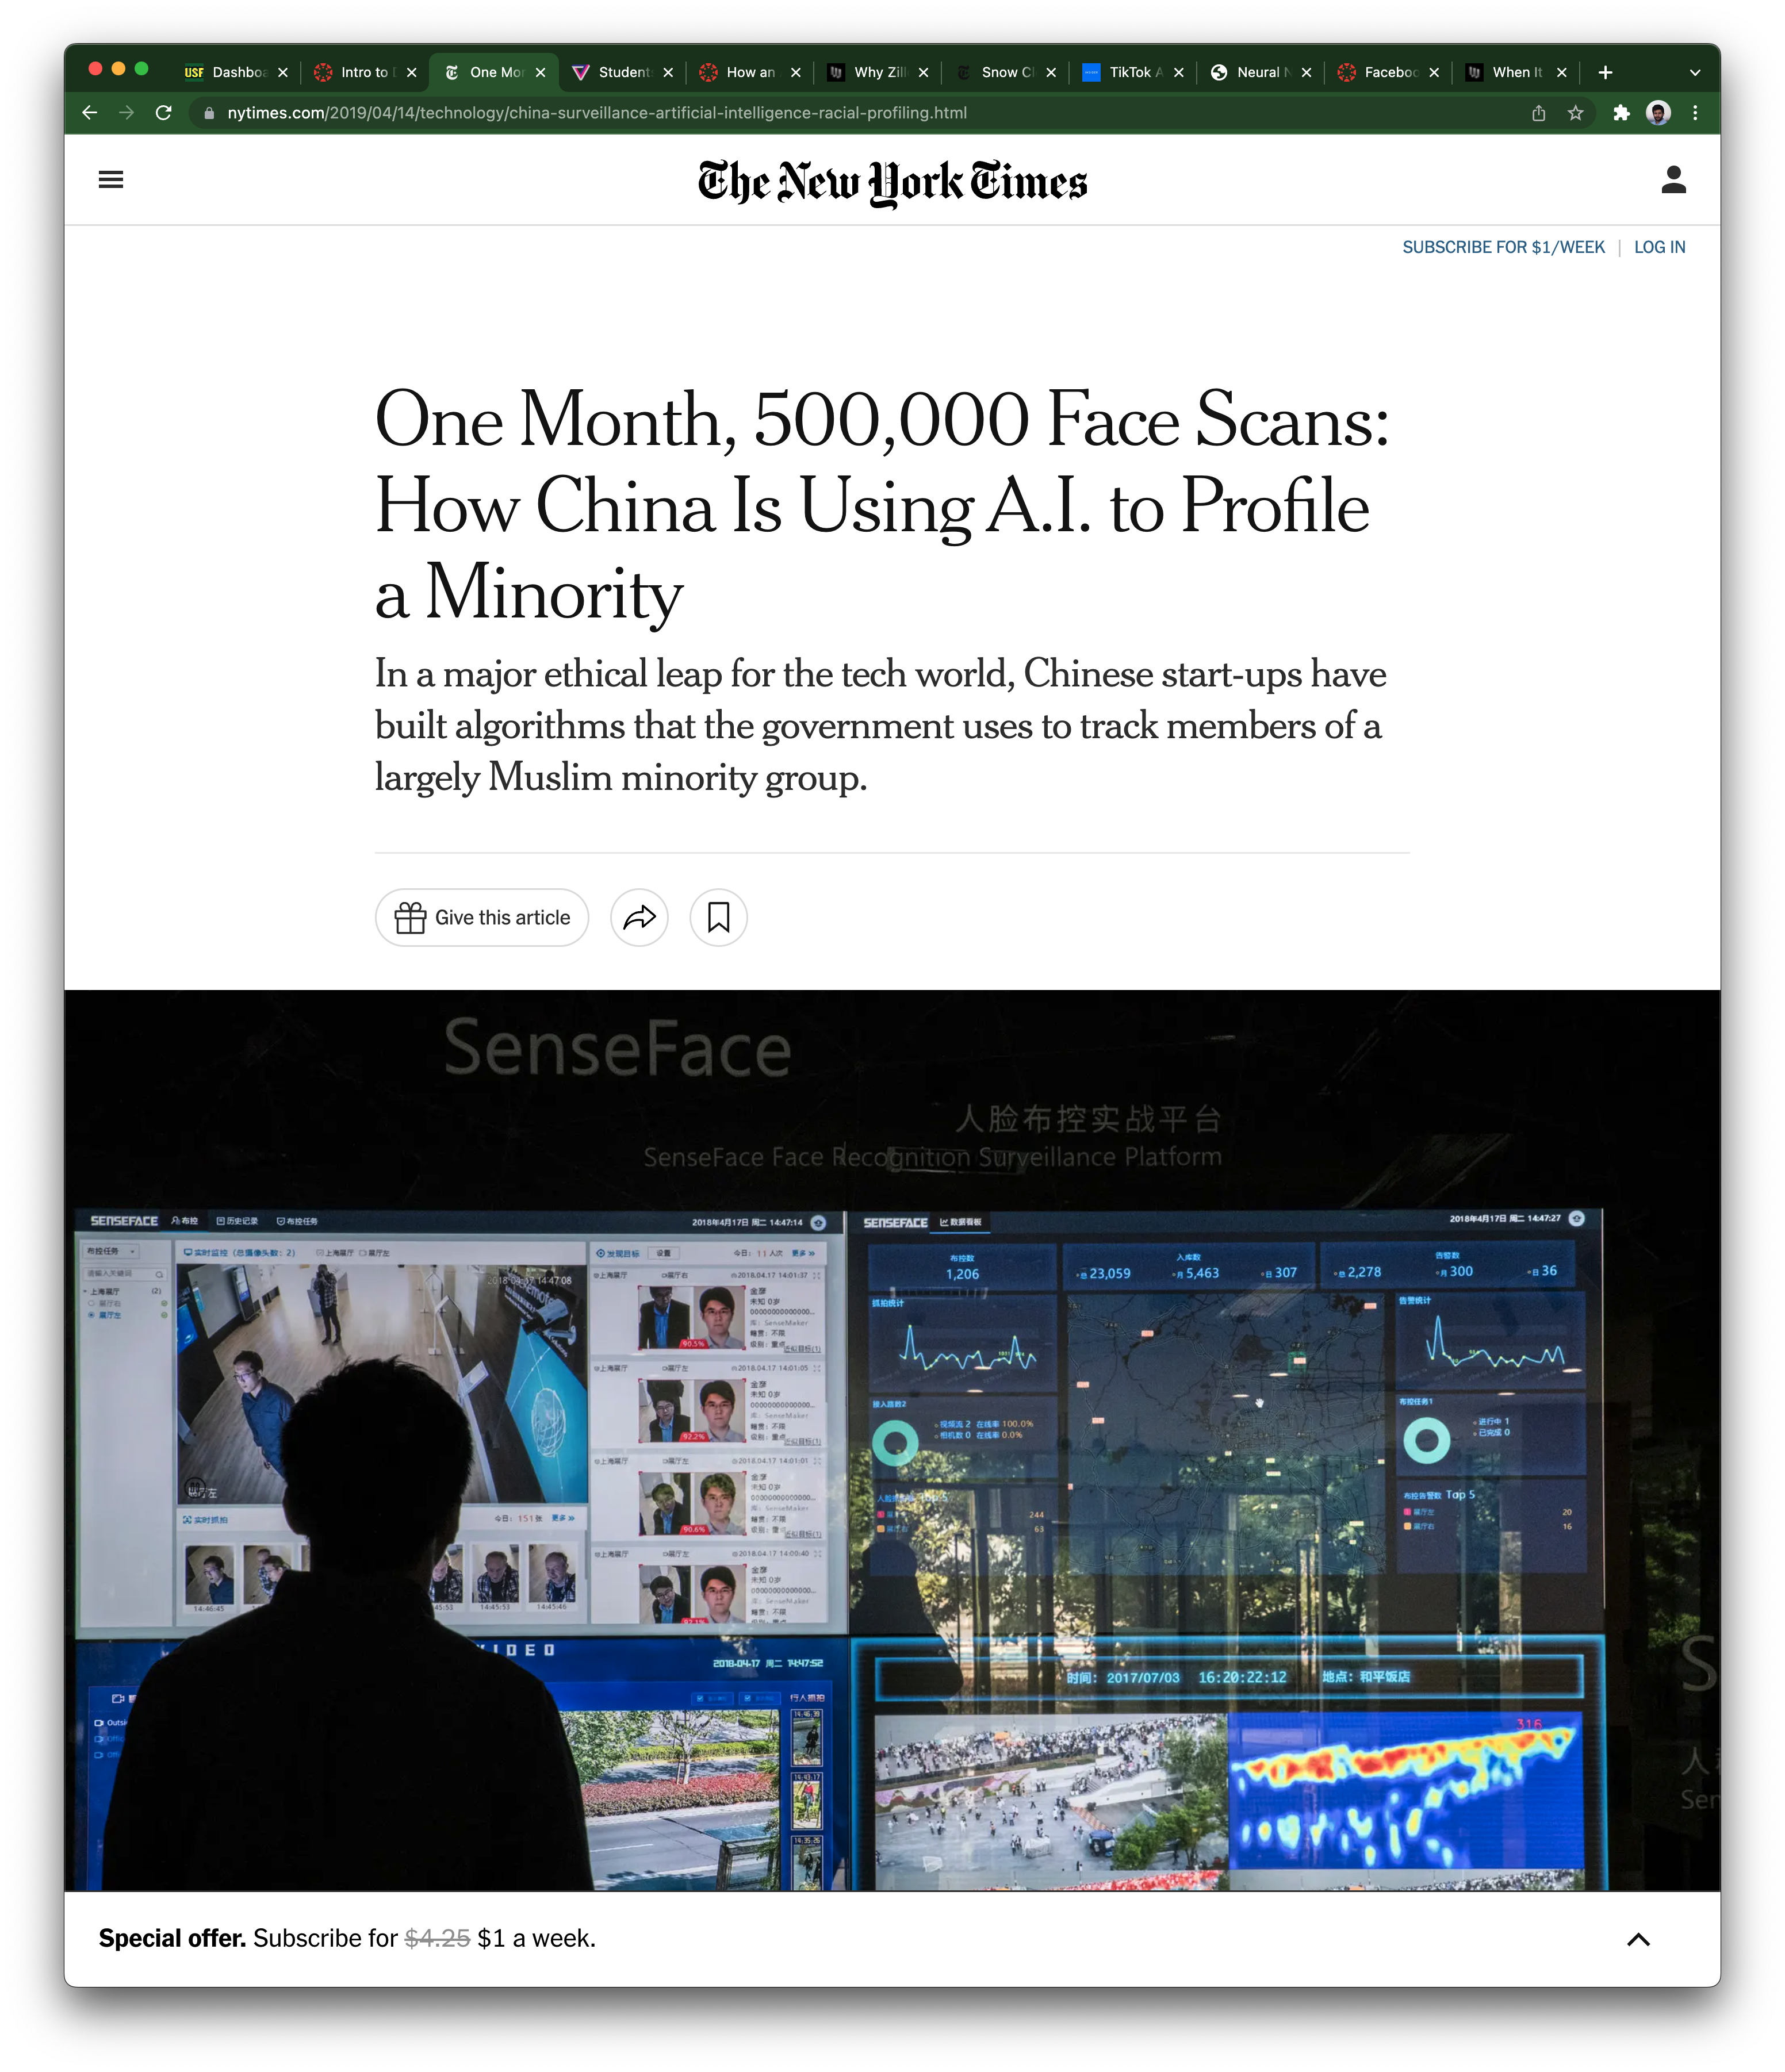
\includegraphics[width=\textwidth]{figures/news/fairer/NYT_social_credit.png}}

\end{column}
\end{columns}
\end{frame}


\begin{frame}[standout]
what is fairness?
\end{frame}

\begin{frame}{fairness}

\begin{columns}
\begin{column}{0.45\textwidth}
\only<1>{A Mulching Proposal}
\only<2->{\strong{The Measure and Mismeasure of Fairness}: A Critical Review of Fair Machine Learning}
\end{column}
\begin{column}{0.55\textwidth}
    \only<+>{\includegraphics[width=\textwidth]{figures/papers/mulching.png}}
    
    \only<+>{\includegraphics[width=\textwidth]{figures/papers/limits.png}}

    \only<+>{
    \centering
    \begin{itemize}
            \item literacy tests
            \item redlining
        \item proxies, like
        \begin{itemize}
        \item zip code
        \item last name
        \end{itemize}
    \end{itemize}}

    \only<+>{
    \centering

    \emph{``\dots there are important cases where even protected group membership itself should be explicitly taken into account to make equitable decisions.''}}
\end{column}
\end{columns}
\end{frame}

\begin{frame}{fairness}
\centering
\visible<+->{To varying degrees, we are \strong{mediators} of ``fair'' or ``equitable'' or ``just'' outcomes.}

\vspace{1em}

\visible<+->{

{\small How can you identify \strong{stakeholders} who might care how the system adjudicates issues?

What is your responsibility regarding a system \strong{after} deployment?}
}

\end{frame}







\end{document}
